\documentclass[10pt]{article}
% Submission to TMLR: \usepackage{tmlr} (anonymous). arXiv: \usepackage[preprint]{tmlr}.
\usepackage[preprint]{tmlr}
%%%%% NEW MATH DEFINITIONS %%%%%

\usepackage{amsmath,amsfonts,bm}

% Mark sections of captions for referring to divisions of figures
\newcommand{\figleft}{{\em (Left)}}
\newcommand{\figcenter}{{\em (Center)}}
\newcommand{\figright}{{\em (Right)}}
\newcommand{\figtop}{{\em (Top)}}
\newcommand{\figbottom}{{\em (Bottom)}}
\newcommand{\captiona}{{\em (a)}}
\newcommand{\captionb}{{\em (b)}}
\newcommand{\captionc}{{\em (c)}}
\newcommand{\captiond}{{\em (d)}}

% Highlight a newly defined term
\newcommand{\newterm}[1]{{\bf #1}}


% Figure reference, lower-case.
\def\figref#1{figure~\ref{#1}}
% Figure reference, capital. For start of sentence
\def\Figref#1{Figure~\ref{#1}}
\def\twofigref#1#2{figures \ref{#1} and \ref{#2}}
\def\quadfigref#1#2#3#4{figures \ref{#1}, \ref{#2}, \ref{#3} and \ref{#4}}
% Section reference, lower-case.
\def\secref#1{section~\ref{#1}}
% Section reference, capital.
\def\Secref#1{Section~\ref{#1}}
% Reference to two sections.
\def\twosecrefs#1#2{sections \ref{#1} and \ref{#2}}
% Reference to three sections.
\def\secrefs#1#2#3{sections \ref{#1}, \ref{#2} and \ref{#3}}
% Reference to an equation, lower-case.
\def\eqref#1{equation~\ref{#1}}
% Reference to an equation, upper case
\def\Eqref#1{Equation~\ref{#1}}
% A raw reference to an equation---avoid using if possible
\def\plaineqref#1{\ref{#1}}
% Reference to a chapter, lower-case.
\def\chapref#1{chapter~\ref{#1}}
% Reference to an equation, upper case.
\def\Chapref#1{Chapter~\ref{#1}}
% Reference to a range of chapters
\def\rangechapref#1#2{chapters\ref{#1}--\ref{#2}}
% Reference to an algorithm, lower-case.
\def\algref#1{algorithm~\ref{#1}}
% Reference to an algorithm, upper case.
\def\Algref#1{Algorithm~\ref{#1}}
\def\twoalgref#1#2{algorithms \ref{#1} and \ref{#2}}
\def\Twoalgref#1#2{Algorithms \ref{#1} and \ref{#2}}
% Reference to a part, lower case
\def\partref#1{part~\ref{#1}}
% Reference to a part, upper case
\def\Partref#1{Part~\ref{#1}}
\def\twopartref#1#2{parts \ref{#1} and \ref{#2}}

\def\ceil#1{\lceil #1 \rceil}
\def\floor#1{\lfloor #1 \rfloor}
\def\1{\bm{1}}
\newcommand{\train}{\mathcal{D}}
\newcommand{\valid}{\mathcal{D_{\mathrm{valid}}}}
\newcommand{\test}{\mathcal{D_{\mathrm{test}}}}

\def\eps{{\epsilon}}


% Random variables
\def\reta{{\textnormal{$\eta$}}}
\def\ra{{\textnormal{a}}}
\def\rb{{\textnormal{b}}}
\def\rc{{\textnormal{c}}}
\def\rd{{\textnormal{d}}}
\def\re{{\textnormal{e}}}
\def\rf{{\textnormal{f}}}
\def\rg{{\textnormal{g}}}
\def\rh{{\textnormal{h}}}
\def\ri{{\textnormal{i}}}
\def\rj{{\textnormal{j}}}
\def\rk{{\textnormal{k}}}
\def\rl{{\textnormal{l}}}
% rm is already a command, just don't name any random variables m
\def\rn{{\textnormal{n}}}
\def\ro{{\textnormal{o}}}
\def\rp{{\textnormal{p}}}
\def\rq{{\textnormal{q}}}
\def\rr{{\textnormal{r}}}
\def\rs{{\textnormal{s}}}
\def\rt{{\textnormal{t}}}
\def\ru{{\textnormal{u}}}
\def\rv{{\textnormal{v}}}
\def\rw{{\textnormal{w}}}
\def\rx{{\textnormal{x}}}
\def\ry{{\textnormal{y}}}
\def\rz{{\textnormal{z}}}

% Random vectors
\def\rvepsilon{{\mathbf{\epsilon}}}
\def\rvtheta{{\mathbf{\theta}}}
\def\rva{{\mathbf{a}}}
\def\rvb{{\mathbf{b}}}
\def\rvc{{\mathbf{c}}}
\def\rvd{{\mathbf{d}}}
\def\rve{{\mathbf{e}}}
\def\rvf{{\mathbf{f}}}
\def\rvg{{\mathbf{g}}}
\def\rvh{{\mathbf{h}}}
\def\rvu{{\mathbf{i}}}
\def\rvj{{\mathbf{j}}}
\def\rvk{{\mathbf{k}}}
\def\rvl{{\mathbf{l}}}
\def\rvm{{\mathbf{m}}}
\def\rvn{{\mathbf{n}}}
\def\rvo{{\mathbf{o}}}
\def\rvp{{\mathbf{p}}}
\def\rvq{{\mathbf{q}}}
\def\rvr{{\mathbf{r}}}
\def\rvs{{\mathbf{s}}}
\def\rvt{{\mathbf{t}}}
\def\rvu{{\mathbf{u}}}
\def\rvv{{\mathbf{v}}}
\def\rvw{{\mathbf{w}}}
\def\rvx{{\mathbf{x}}}
\def\rvy{{\mathbf{y}}}
\def\rvz{{\mathbf{z}}}

% Elements of random vectors
\def\erva{{\textnormal{a}}}
\def\ervb{{\textnormal{b}}}
\def\ervc{{\textnormal{c}}}
\def\ervd{{\textnormal{d}}}
\def\erve{{\textnormal{e}}}
\def\ervf{{\textnormal{f}}}
\def\ervg{{\textnormal{g}}}
\def\ervh{{\textnormal{h}}}
\def\ervi{{\textnormal{i}}}
\def\ervj{{\textnormal{j}}}
\def\ervk{{\textnormal{k}}}
\def\ervl{{\textnormal{l}}}
\def\ervm{{\textnormal{m}}}
\def\ervn{{\textnormal{n}}}
\def\ervo{{\textnormal{o}}}
\def\ervp{{\textnormal{p}}}
\def\ervq{{\textnormal{q}}}
\def\ervr{{\textnormal{r}}}
\def\ervs{{\textnormal{s}}}
\def\ervt{{\textnormal{t}}}
\def\ervu{{\textnormal{u}}}
\def\ervv{{\textnormal{v}}}
\def\ervw{{\textnormal{w}}}
\def\ervx{{\textnormal{x}}}
\def\ervy{{\textnormal{y}}}
\def\ervz{{\textnormal{z}}}

% Random matrices
\def\rmA{{\mathbf{A}}}
\def\rmB{{\mathbf{B}}}
\def\rmC{{\mathbf{C}}}
\def\rmD{{\mathbf{D}}}
\def\rmE{{\mathbf{E}}}
\def\rmF{{\mathbf{F}}}
\def\rmG{{\mathbf{G}}}
\def\rmH{{\mathbf{H}}}
\def\rmI{{\mathbf{I}}}
\def\rmJ{{\mathbf{J}}}
\def\rmK{{\mathbf{K}}}
\def\rmL{{\mathbf{L}}}
\def\rmM{{\mathbf{M}}}
\def\rmN{{\mathbf{N}}}
\def\rmO{{\mathbf{O}}}
\def\rmP{{\mathbf{P}}}
\def\rmQ{{\mathbf{Q}}}
\def\rmR{{\mathbf{R}}}
\def\rmS{{\mathbf{S}}}
\def\rmT{{\mathbf{T}}}
\def\rmU{{\mathbf{U}}}
\def\rmV{{\mathbf{V}}}
\def\rmW{{\mathbf{W}}}
\def\rmX{{\mathbf{X}}}
\def\rmY{{\mathbf{Y}}}
\def\rmZ{{\mathbf{Z}}}

% Elements of random matrices
\def\ermA{{\textnormal{A}}}
\def\ermB{{\textnormal{B}}}
\def\ermC{{\textnormal{C}}}
\def\ermD{{\textnormal{D}}}
\def\ermE{{\textnormal{E}}}
\def\ermF{{\textnormal{F}}}
\def\ermG{{\textnormal{G}}}
\def\ermH{{\textnormal{H}}}
\def\ermI{{\textnormal{I}}}
\def\ermJ{{\textnormal{J}}}
\def\ermK{{\textnormal{K}}}
\def\ermL{{\textnormal{L}}}
\def\ermM{{\textnormal{M}}}
\def\ermN{{\textnormal{N}}}
\def\ermO{{\textnormal{O}}}
\def\ermP{{\textnormal{P}}}
\def\ermQ{{\textnormal{Q}}}
\def\ermR{{\textnormal{R}}}
\def\ermS{{\textnormal{S}}}
\def\ermT{{\textnormal{T}}}
\def\ermU{{\textnormal{U}}}
\def\ermV{{\textnormal{V}}}
\def\ermW{{\textnormal{W}}}
\def\ermX{{\textnormal{X}}}
\def\ermY{{\textnormal{Y}}}
\def\ermZ{{\textnormal{Z}}}

% Vectors
\def\vzero{{\bm{0}}}
\def\vone{{\bm{1}}}
\def\vmu{{\bm{\mu}}}
\def\vtheta{{\bm{\theta}}}
\def\va{{\bm{a}}}
\def\vb{{\bm{b}}}
\def\vc{{\bm{c}}}
\def\vd{{\bm{d}}}
\def\ve{{\bm{e}}}
\def\vf{{\bm{f}}}
\def\vg{{\bm{g}}}
\def\vh{{\bm{h}}}
\def\vi{{\bm{i}}}
\def\vj{{\bm{j}}}
\def\vk{{\bm{k}}}
\def\vl{{\bm{l}}}
\def\vm{{\bm{m}}}
\def\vn{{\bm{n}}}
\def\vo{{\bm{o}}}
\def\vp{{\bm{p}}}
\def\vq{{\bm{q}}}
\def\vr{{\bm{r}}}
\def\vs{{\bm{s}}}
\def\vt{{\bm{t}}}
\def\vu{{\bm{u}}}
\def\vv{{\bm{v}}}
\def\vw{{\bm{w}}}
\def\vx{{\bm{x}}}
\def\vy{{\bm{y}}}
\def\vz{{\bm{z}}}

% Elements of vectors
\def\evalpha{{\alpha}}
\def\evbeta{{\beta}}
\def\evepsilon{{\epsilon}}
\def\evlambda{{\lambda}}
\def\evomega{{\omega}}
\def\evmu{{\mu}}
\def\evpsi{{\psi}}
\def\evsigma{{\sigma}}
\def\evtheta{{\theta}}
\def\eva{{a}}
\def\evb{{b}}
\def\evc{{c}}
\def\evd{{d}}
\def\eve{{e}}
\def\evf{{f}}
\def\evg{{g}}
\def\evh{{h}}
\def\evi{{i}}
\def\evj{{j}}
\def\evk{{k}}
\def\evl{{l}}
\def\evm{{m}}
\def\evn{{n}}
\def\evo{{o}}
\def\evp{{p}}
\def\evq{{q}}
\def\evr{{r}}
\def\evs{{s}}
\def\evt{{t}}
\def\evu{{u}}
\def\evv{{v}}
\def\evw{{w}}
\def\evx{{x}}
\def\evy{{y}}
\def\evz{{z}}

% Matrix
\def\mA{{\bm{A}}}
\def\mB{{\bm{B}}}
\def\mC{{\bm{C}}}
\def\mD{{\bm{D}}}
\def\mE{{\bm{E}}}
\def\mF{{\bm{F}}}
\def\mG{{\bm{G}}}
\def\mH{{\bm{H}}}
\def\mI{{\bm{I}}}
\def\mJ{{\bm{J}}}
\def\mK{{\bm{K}}}
\def\mL{{\bm{L}}}
\def\mM{{\bm{M}}}
\def\mN{{\bm{N}}}
\def\mO{{\bm{O}}}
\def\mP{{\bm{P}}}
\def\mQ{{\bm{Q}}}
\def\mR{{\bm{R}}}
\def\mS{{\bm{S}}}
\def\mT{{\bm{T}}}
\def\mU{{\bm{U}}}
\def\mV{{\bm{V}}}
\def\mW{{\bm{W}}}
\def\mX{{\bm{X}}}
\def\mY{{\bm{Y}}}
\def\mZ{{\bm{Z}}}
\def\mBeta{{\bm{\beta}}}
\def\mPhi{{\bm{\Phi}}}
\def\mLambda{{\bm{\Lambda}}}
\def\mSigma{{\bm{\Sigma}}}

% Tensor
\DeclareMathAlphabet{\mathsfit}{\encodingdefault}{\sfdefault}{m}{sl}
\SetMathAlphabet{\mathsfit}{bold}{\encodingdefault}{\sfdefault}{bx}{n}
\newcommand{\tens}[1]{\bm{\mathsfit{#1}}}
\def\tA{{\tens{A}}}
\def\tB{{\tens{B}}}
\def\tC{{\tens{C}}}
\def\tD{{\tens{D}}}
\def\tE{{\tens{E}}}
\def\tF{{\tens{F}}}
\def\tG{{\tens{G}}}
\def\tH{{\tens{H}}}
\def\tI{{\tens{I}}}
\def\tJ{{\tens{J}}}
\def\tK{{\tens{K}}}
\def\tL{{\tens{L}}}
\def\tM{{\tens{M}}}
\def\tN{{\tens{N}}}
\def\tO{{\tens{O}}}
\def\tP{{\tens{P}}}
\def\tQ{{\tens{Q}}}
\def\tR{{\tens{R}}}
\def\tS{{\tens{S}}}
\def\tT{{\tens{T}}}
\def\tU{{\tens{U}}}
\def\tV{{\tens{V}}}
\def\tW{{\tens{W}}}
\def\tX{{\tens{X}}}
\def\tY{{\tens{Y}}}
\def\tZ{{\tens{Z}}}


% Graph
\def\gA{{\mathcal{A}}}
\def\gB{{\mathcal{B}}}
\def\gC{{\mathcal{C}}}
\def\gD{{\mathcal{D}}}
\def\gE{{\mathcal{E}}}
\def\gF{{\mathcal{F}}}
\def\gG{{\mathcal{G}}}
\def\gH{{\mathcal{H}}}
\def\gI{{\mathcal{I}}}
\def\gJ{{\mathcal{J}}}
\def\gK{{\mathcal{K}}}
\def\gL{{\mathcal{L}}}
\def\gM{{\mathcal{M}}}
\def\gN{{\mathcal{N}}}
\def\gO{{\mathcal{O}}}
\def\gP{{\mathcal{P}}}
\def\gQ{{\mathcal{Q}}}
\def\gR{{\mathcal{R}}}
\def\gS{{\mathcal{S}}}
\def\gT{{\mathcal{T}}}
\def\gU{{\mathcal{U}}}
\def\gV{{\mathcal{V}}}
\def\gW{{\mathcal{W}}}
\def\gX{{\mathcal{X}}}
\def\gY{{\mathcal{Y}}}
\def\gZ{{\mathcal{Z}}}

% Sets
\def\sA{{\mathbb{A}}}
\def\sB{{\mathbb{B}}}
\def\sC{{\mathbb{C}}}
\def\sD{{\mathbb{D}}}
% Don't use a set called E, because this would be the same as our symbol
% for expectation.
\def\sF{{\mathbb{F}}}
\def\sG{{\mathbb{G}}}
\def\sH{{\mathbb{H}}}
\def\sI{{\mathbb{I}}}
\def\sJ{{\mathbb{J}}}
\def\sK{{\mathbb{K}}}
\def\sL{{\mathbb{L}}}
\def\sM{{\mathbb{M}}}
\def\sN{{\mathbb{N}}}
\def\sO{{\mathbb{O}}}
\def\sP{{\mathbb{P}}}
\def\sQ{{\mathbb{Q}}}
\def\sR{{\mathbb{R}}}
\def\sS{{\mathbb{S}}}
\def\sT{{\mathbb{T}}}
\def\sU{{\mathbb{U}}}
\def\sV{{\mathbb{V}}}
\def\sW{{\mathbb{W}}}
\def\sX{{\mathbb{X}}}
\def\sY{{\mathbb{Y}}}
\def\sZ{{\mathbb{Z}}}

% Entries of a matrix
\def\emLambda{{\Lambda}}
\def\emA{{A}}
\def\emB{{B}}
\def\emC{{C}}
\def\emD{{D}}
\def\emE{{E}}
\def\emF{{F}}
\def\emG{{G}}
\def\emH{{H}}
\def\emI{{I}}
\def\emJ{{J}}
\def\emK{{K}}
\def\emL{{L}}
\def\emM{{M}}
\def\emN{{N}}
\def\emO{{O}}
\def\emP{{P}}
\def\emQ{{Q}}
\def\emR{{R}}
\def\emS{{S}}
\def\emT{{T}}
\def\emU{{U}}
\def\emV{{V}}
\def\emW{{W}}
\def\emX{{X}}
\def\emY{{Y}}
\def\emZ{{Z}}
\def\emSigma{{\Sigma}}

% entries of a tensor
% Same font as tensor, without \bm wrapper
\newcommand{\etens}[1]{\mathsfit{#1}}
\def\etLambda{{\etens{\Lambda}}}
\def\etA{{\etens{A}}}
\def\etB{{\etens{B}}}
\def\etC{{\etens{C}}}
\def\etD{{\etens{D}}}
\def\etE{{\etens{E}}}
\def\etF{{\etens{F}}}
\def\etG{{\etens{G}}}
\def\etH{{\etens{H}}}
\def\etI{{\etens{I}}}
\def\etJ{{\etens{J}}}
\def\etK{{\etens{K}}}
\def\etL{{\etens{L}}}
\def\etM{{\etens{M}}}
\def\etN{{\etens{N}}}
\def\etO{{\etens{O}}}
\def\etP{{\etens{P}}}
\def\etQ{{\etens{Q}}}
\def\etR{{\etens{R}}}
\def\etS{{\etens{S}}}
\def\etT{{\etens{T}}}
\def\etU{{\etens{U}}}
\def\etV{{\etens{V}}}
\def\etW{{\etens{W}}}
\def\etX{{\etens{X}}}
\def\etY{{\etens{Y}}}
\def\etZ{{\etens{Z}}}

% The true underlying data generating distribution
\newcommand{\pdata}{p_{\rm{data}}}
% The empirical distribution defined by the training set
\newcommand{\ptrain}{\hat{p}_{\rm{data}}}
\newcommand{\Ptrain}{\hat{P}_{\rm{data}}}
% The model distribution
\newcommand{\pmodel}{p_{\rm{model}}}
\newcommand{\Pmodel}{P_{\rm{model}}}
\newcommand{\ptildemodel}{\tilde{p}_{\rm{model}}}
% Stochastic autoencoder distributions
\newcommand{\pencode}{p_{\rm{encoder}}}
\newcommand{\pdecode}{p_{\rm{decoder}}}
\newcommand{\precons}{p_{\rm{reconstruct}}}

\newcommand{\laplace}{\mathrm{Laplace}} % Laplace distribution

\newcommand{\E}{\mathbb{E}}
\newcommand{\Ls}{\mathcal{L}}
\newcommand{\R}{\mathbb{R}}
\newcommand{\emp}{\tilde{p}}
\newcommand{\lr}{\alpha}
\newcommand{\reg}{\lambda}
\newcommand{\rect}{\mathrm{rectifier}}
\newcommand{\softmax}{\mathrm{softmax}}
\newcommand{\sigmoid}{\sigma}
\newcommand{\softplus}{\zeta}
\newcommand{\KL}{D_{\mathrm{KL}}}
\newcommand{\Var}{\mathrm{Var}}
\newcommand{\standarderror}{\mathrm{SE}}
\newcommand{\Cov}{\mathrm{Cov}}
% Wolfram Mathworld says $L^2$ is for function spaces and $\ell^2$ is for vectors
% But then they seem to use $L^2$ for vectors throughout the site, and so does
% wikipedia.
\newcommand{\normlzero}{L^0}
\newcommand{\normlone}{L^1}
\newcommand{\normltwo}{L^2}
\newcommand{\normlp}{L^p}
\newcommand{\normmax}{L^\infty}

\newcommand{\parents}{Pa} % See usage in notation.tex. Chosen to match Daphne's book.

\DeclareMathOperator*{\argmax}{arg\,max}
\DeclareMathOperator*{\argmin}{arg\,min}

\DeclareMathOperator{\sign}{sign}
\DeclareMathOperator{\Tr}{Tr}
\let\ab\allowbreak

\usepackage{hyperref}
\usepackage{url}
\usepackage{booktabs}
\usepackage{multirow}
\usepackage{graphicx}
\usepackage{xcolor}
\newcommand{\todo}[1]{\textcolor{red}{[TODO: #1]}}

\title{The Cost of Being Live: How Much Future Context\\ Real-Time Behavior Classifiers Need, in Mice and Flies}

\author{\name Ava Sajjadi \email avasajjadi2019@gmail.com \\
      \addr \todo{affiliation}}

\def\month{MM}
\def\year{YYYY}
\def\openreview{\url{https://openreview.net/forum?id=XXXX}}

\begin{document}
\maketitle

\begin{abstract}
Closed-loop neuroscience experiments must label behavior while it happens, yet behavior classifiers are usually built and benchmarked offline, with access to future frames: the CalMS21 baselines, for example, see 100 frames ahead. We measure what being live costs. One temporal network, with the same 63-frame (2.1\,s) window, is trained and scored with the window moved from all-past (live) to centred, at six delays and three seeds each, for 11 behaviors in three datasets (mouse social behavior, fly aggression, fly courtship). Being live costs mice about 0.01 class-averaged F1, about the seed spread, but costs some fly behaviors a great deal: fly lunge rises from 0.39 to 0.72 F1 with a 0.1\,s wait. Across behaviors, a 0.1--0.2\,s wait recovers most of what the full centred window gives, and the gain from waiting is larger for behaviors with shorter bouts (Spearman $\rho=-0.73$, exact permutation $p=0.015$, declared before running). We then test this claim against itself: it survives dropping any one or two behaviors, but among fly behaviors alone it is weak ($\rho=-0.33$, $p=0.43$), so bout length is confounded with species. To separate the two, we compute the Bayes-optimal fixed-lag decoder for simulated behaviors whose bout lengths we control. Its gain from waiting falls for bouts longer than a few tenths of a second, for every bout shape and noise level tried, and a short wait captures nearly all of the centred-window gain for short bouts. Fly lunges gain more than three times what this model allows, which points to evidence that arrives after a bout begins rather than to noise alone. Finally, the live classifier itself (EthoLive) runs at 75 frames per second on a laptop and scores 0.847 class-averaged F1 on the CalMS21 Task~1 test set, within 0.02 of the best offline challenge entry; every look at every test split is recorded in a ledger that we publish.
\end{abstract}

\section{Introduction}

Automated behavior analysis now runs from pose estimation \citep{mathis2018deeplabcut,pereira2022sleap} to supervised \citep{segalin2021mars,goodwin2024simba} or unsupervised \citep{weinreb2024keypointmoseq} behavior models. Most of this work is offline. A recorded session is processed afterwards, and the classifier may look at frames both before and after the frame it labels; the CalMS21 benchmark baselines use 100 past and 100 future frames and state that models need not be causal \citep{sun2021calms21}. Closed-loop experiments, such as stimulating a circuit when an attack begins, cannot wait for the future: they need a label within a fraction of a second, from the past only \citep{schweihoff2021deeplabstream,kane2020realtime,yamanouchi2026yoru}.

How much accuracy does that constraint cost, and for which behaviors? The answer decides whether a lab can reuse an offline classifier for closed-loop work, and how long a stimulator should wait before acting. Classical results on hidden Markov models say that the value of extra lookahead decays quickly with the lag \citep{shue1998exponential,venkat2016lookahead}, but behavior classifiers are learned, behaviors last from a tenth of a second to minutes, and the cost of being live has, to our knowledge, not been measured across behaviors with the model held fixed.

\paragraph{Contributions.}
\begin{itemize}
  \item \textbf{A controlled measurement} (Sections~\ref{sec:setup}--\ref{sec:results}). One network and one 63-frame window, moved from all-past to centred in six steps, with labels and training otherwise unchanged; 11 behaviors in three datasets and two species, three seeds per setting, validation data only. The hypothesis and test were written into the script before it ran.
  \item \textbf{A finding with its limits} (Section~\ref{sec:results}). Being live costs mice almost nothing and some short fly behaviors a lot; a 0.1--0.2\,s wait recovers most of the centred-window gain. Shorter behaviors gain more ($\rho=-0.73$, $p=0.015$), but a drop-out analysis shows the trend rests on the mouse--fly contrast and is not significant within flies.
  \item \textbf{A Bayes-optimal reference} (Section~\ref{sec:synthetic}). For simulated behaviors with controlled bout lengths, the exact fixed-lag posterior shows how much waiting can help when the only problem is per-frame noise. It reproduces the falling side of the measured trend, and shows that the largest measured gain (fly lunge) is not explained by noise alone.
  \item \textbf{A live classifier and an auditable protocol} (Section~\ref{sec:etholive}). EthoLive runs at 75 frames per second end to end on a laptop and reaches 0.847 class-averaged F1 on the CalMS21 Task~1 test set (offline baseline 0.793, challenge winner 0.864). We publish a ledger of every look at every test split, including the cases where validation overstated test performance.
\end{itemize}

\section{Related work}

\paragraph{Pose-based behavior classification.} MARS \citep{segalin2021mars} introduced the pose and behavior pipeline whose keypoints CalMS21 uses. SimBA \citep{goodwin2024simba} trains per-behavior classifiers on pose features. CalMS21 and the MABe challenge \citep{sun2021calms21} standardized evaluation; their Task~1 baselines see 100 past and 100 future frames (with a skip factor of 2), reaching 0.793 class-averaged F1, 0.829 with task programming, and 0.864 for the challenge winner. Fly vs.\ Fly \citep{eyjolfsdottir2014flyvsfly} provides the fly aggression and courtship labels we use.

\paragraph{Real-time and closed-loop tools.} DeepLabStream \citep{schweihoff2021deeplabstream} and real-time DeepLabCut \citep{kane2020realtime} trigger on pose events with low latency. YORU \citep{yamanouchi2026yoru} detects behaviors as objects in single frames for closed-loop control. These systems report latency; we ask what accuracy the causal constraint itself costs, with the model held fixed.

\paragraph{Lookahead, smoothing and delay.} For hidden Markov models, filters and fixed-lag smoothers forget their initial conditions exponentially fast, so the benefit of further lag decays quickly \citep{shue1998exponential}. Information-theoretic work characterizes estimation and coding with finite lookahead \citep{venkat2016lookahead,asnani2013lookahead}. Behavior bouts are not geometric, which motivates hidden semi-Markov models \citep{yu2010hsmm}. Section~\ref{sec:synthetic} uses exact fixed-lag decoding of such models as a reference for the learned classifier.

\paragraph{Evaluation practice.} Reusing a test set inflates reported performance \citep{dwork2015reusable,recht2019imagenet}, and conclusions drawn from data can hinge on a few observations \citep{broderick2020amip}. We count and publish every look at each test split, and test the main claim by dropping behaviors and datasets.

\section{Setup}
\label{sec:setup}

\paragraph{Model.} Behavior logits at each frame are the sum of a \emph{frame branch}, a linear model on that frame's pose features (120 for mice), initialised from a logistic regression, and a \emph{memory branch}, a dilated 1D convolution (kernel 3, dilations 1, 2, 4, 8, 16, width 64, dropout 0.1) whose receptive field is 63 frames (2.1\,s at 30\,fps). Features come from a fixed, non-learned pipeline: identity-swap repair, per-keypoint One-Euro filtering \citep{casiez2012oneeuro}, velocities and accelerations, body axis and bend, and inter-animal geometry. Training uses AdamW (learning rate $10^{-3}$, weight decay $10^{-4}$), batches of 32 windows of 256 frames, 300 steps per epoch for up to 40 epochs, and class-weighted cross-entropy; each network keeps its epoch with the best validation class-averaged F1. Three seeds are averaged in probability (the ``team'').

\paragraph{Moving the window.} With delay $K$, the label of frame $t$ is predicted at frame $t+K$, so the memory branch sees frames $t-62+K$ to $t+K$: $K=0$ is live (62 past frames) and $K=31$ is centred (31 past, 31 future), i.e.\ an offline model with the same context and the same number of weights. The frame branch always reads frame $t$ itself, so only the memory window moves. We use $K \in \{0,3,6,10,15,31\}$ (0 to 1.03\,s).

\paragraph{Data.} \emph{Mouse}: CalMS21 Task~1 \citep{sun2021calms21}, 56 training and 14 validation sessions (attack, investigation, mount). \emph{Fly aggression}: Fly vs.\ Fly Aggression and Boy-meets-boy at 30\,fps with courtship hard negatives \citep{eyjolfsdottir2014flyvsfly}; three folds, each holding out one Aggression movie pair and one Boy-meets-boy movie (lunge, wing threat, tussle, hold). \emph{Fly courtship}: the Courtship training half in two folds (wing extension, circling, attempted copulation, copulation). Fly features are computed from our own pose network's points. All numbers in Sections~\ref{sec:results} and \ref{sec:synthetic} are validation numbers; no test split was used.

\paragraph{Measure and declared test.} For each behavior we report the team's F1 at each $K$, averaged over folds, and the gain $\Delta(K) = \mathrm{F1}(K) - \mathrm{F1}(0)$. A behavior's duration is the median length of its bouts in the training labels. Before running, we declared one test: the Spearman correlation across the 11 behaviors between median duration and $\Delta(6)$ and $\Delta(31)$, with an exact permutation $p$-value, and stated that 11 points can only give a hint.

\section{Results: what being live costs}
\label{sec:results}

\begin{figure}[t]
\centering
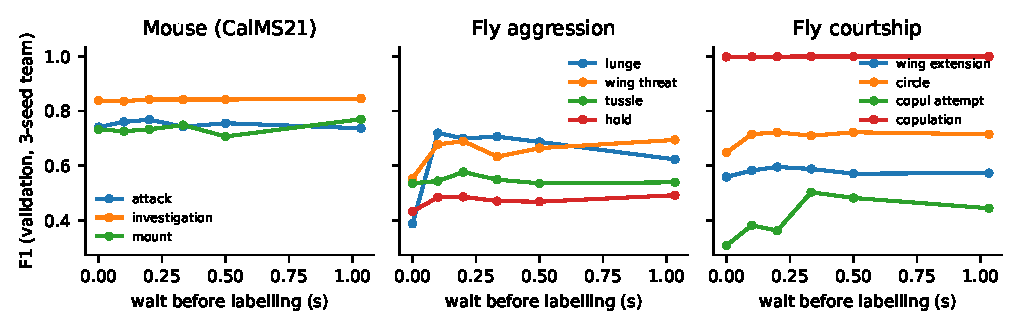
\includegraphics[width=\linewidth]{figures/f1_vs_wait.pdf}
\caption{F1 against the wait before labelling, for one network whose 63-frame window is moved from all-past (0\,s) to centred (1.03\,s). Validation data; three-seed team; fly curves are means over folds.}
\label{fig:curves}
\end{figure}

\begin{table}[t]
\centering
\caption{F1 by wait $K$ (frames at 30\,fps) and gain over live. Validation, three-seed team, mean over folds. Bout: median bout length in the training labels.}
\label{tab:lookahead}
\begin{tabular}{llrccccccr}
\toprule
Data & Behavior & Bout (s) & $K{=}0$ & 3 & 6 & 10 & 15 & 31 & $\Delta(6)$ \\
\midrule
Mouse & attack & 1.45 & .741 & .760 & .768 & .742 & .755 & .737 & +.027 \\
 & investigation & 1.10 & .838 & .836 & .842 & .842 & .842 & .845 & +.004 \\
 & mount & 2.07 & .733 & .726 & .733 & .748 & .707 & .770 & +.000 \\
\midrule
Fly aggression & lunge & 0.13 & .388 & .719 & .700 & .706 & .687 & .623 & +.312 \\
 & wing threat & 0.63 & .553 & .678 & .690 & .634 & .664 & .694 & +.136 \\
 & tussle & 0.23 & .536 & .544 & .577 & .549 & .536 & .539 & +.041 \\
 & hold & 0.17 & .433 & .485 & .486 & .471 & .469 & .492 & +.054 \\
\midrule
Fly courtship & wing extension & 0.40 & .559 & .583 & .596 & .588 & .571 & .573 & +.036 \\
 & circling & 0.43 & .648 & .715 & .722 & .710 & .722 & .715 & +.074 \\
 & attempted copulation & 0.27 & .309 & .383 & .363 & .503 & .482 & .445 & +.054 \\
 & copulation & 1042 & .998 & .998 & .998 & .999 & .999 & .999 & +.001 \\
\bottomrule
\end{tabular}
\end{table}

\paragraph{Mice lose little; some fly behaviors lose a lot.} Figure~\ref{fig:curves} and Table~\ref{tab:lookahead} show the curves. For mice, class-averaged F1 moves from 0.771 live to 0.781 at $K=6$ and 0.784 centred, a change about the size of the seed spread; the largest per-class change is mount at $K=31$ (+0.037). Fly lunge, the shortest behavior (median bout 0.13\,s, 4 frames), rises from 0.388 to 0.719 with a 0.1\,s wait, and the jump appears in each of the three folds (0.40 to 0.66, 0.37 to 0.78, and 0.40 to 0.73 at $K=3$). Wing threat and circling gain 0.07 to 0.14.

\paragraph{A short wait is enough.} The centred window beats a 0.2\,s wait by more than 0.01 for only two behaviors, mount (+0.037) and attempted copulation (+0.082, whose best value is at $K=10$). For lunge it is clearly worse (0.623 against 0.700), consistent with a fixed-size window spending its context on the future at the expense of the past.

\paragraph{The declared test.} Across the 11 behaviors, the gain from a 0.2\,s wait is larger for shorter behaviors: Spearman $\rho=-0.73$, exact permutation $p=0.015$. For the centred window the association is weaker ($\rho=-0.55$, $p=0.087$); at $K=3$ and $K=10$ it is $-0.65$ ($p=0.039$) and $-0.66$ ($p=0.029$).

\begin{table}[t]
\centering
\caption{How fragile is the duration trend? Spearman $\rho$ between median bout length and $\Delta(6)$ after removing behaviors or datasets. For subset removals, the worst case over all subsets of that size.}
\label{tab:robust}
\begin{tabular}{lccc}
\toprule
Removed & Behaviors left & $\rho$ & $p$ \\
\midrule
nothing & 11 & $-0.73$ & 0.015 \\
any 1 behavior (worst of 11) & 10 & $-0.64$ & -- \\
any 2 behaviors (worst of 55) & 9 & $-0.52$ & -- \\
any 3 behaviors (worst of 165) & 8 & $-0.31$ & -- \\
fly courtship & 7 & $-0.86$ & 0.024 \\
fly aggression & 7 & $-0.82$ & 0.034 \\
mouse (flies only) & 8 & $-0.33$ & 0.43 \\
\midrule
within mouse / aggression / courtship & 3 / 4 / 4 & $-0.50$ / $-0.40$ / $-0.40$ & -- \\
\bottomrule
\end{tabular}
\end{table}

\paragraph{Testing the claim against itself.} Eleven points from three datasets can mislead, so we removed behaviors and datasets and recomputed the correlation (Table~\ref{tab:robust}), in the spirit of asking whether dropping a little data changes a conclusion \citep{broderick2020amip}. The trend survives the removal of any one or two behaviors ($\rho \le -0.52$ in all 66 cases). Ten of the 165 three-behavior removals weaken it beyond $-0.5$; the worst ($-0.31$) removes lunge and two mouse behaviors. Removing either fly dataset leaves it intact. Removing the mouse, however, leaves $\rho=-0.33$ ($p=0.43$): among fly behaviors, bout length alone does not predict the gain, and wing threat (0.63\,s) gains far more than its length would suggest. Within each dataset the sign is negative, but three or four behaviors cannot support a test. The honest summary is that being live costs long mouse behaviors little and some short fly behaviors much, and that species, frame-level evidence and bout length are not separated by these data. The next section separates them in simulation.

\section{What the best possible decoder would gain}
\label{sec:synthetic}

If a behavior were a hidden on/off state seen through per-frame noise, how much could waiting help, and how would that depend on bout length? We answer exactly for simulated behaviors, with the design declared in the script before running.

\paragraph{Simulation.} A behavior alternates between bouts and gaps (an alternating renewal process at 30\,fps, 200{,}000 frames per setting). Bouts follow one of three phase-type shapes, all matched on median length $m$: \emph{geometric} (memoryless, the shape behind classic HMM results), \emph{Erlang-4} (regular bouts), and a \emph{mixture} of two geometric lengths (80\% short, 20\% five times longer: a heavy right tail). Gaps are geometric with mean four times the mean bout, so the behavior fills about 20\% of frames. Each frame yields a reading $y_t \sim \mathcal{N}(d\cdot \mathrm{on}_t, 1)$. Because the bout shapes are phase-type, the process is a hidden Markov chain over a few phases, and the exact fixed-lag posterior $P(\mathrm{on}_t \mid y_{1:t+K})$ follows from a forward filter and a $K$-step backward pass. We report F1 at the best threshold for each $K$, for $m$ from 2 to 64 frames (0.07 to 2.1\,s), with $d=1$ for all shapes and, for the geometric shape, also $d=0.5$ and $d=2$.

\begin{figure}[t]
\centering
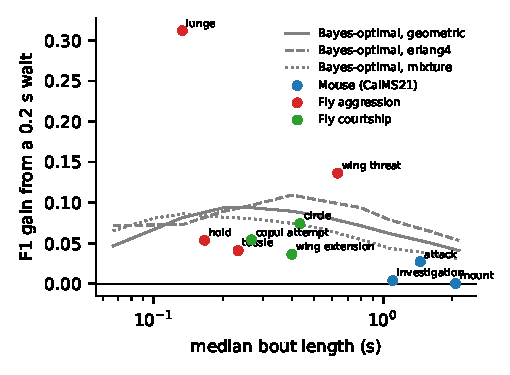
\includegraphics[width=0.6\linewidth]{figures/gain_vs_bout.pdf}
\caption{Gain in F1 from a 0.2\,s wait against median bout length. Points: the learned network on validation data (Table~\ref{tab:lookahead}; copulation, 17\,min, not shown). Lines: the Bayes-optimal fixed-lag decoder on simulated behaviors with three bout shapes and per-frame separation $d=1$.}
\label{fig:gain}
\end{figure}

\paragraph{Results.} Three things hold in every setting we simulated. (i) The optimal gain from waiting is an inverted U in bout length: very short bouts are hard to detect even with hindsight, and long bouts are easy to detect without it. At $d=1$ the gain from a 0.2\,s wait peaks at 0.09--0.11 for bouts of 0.2--0.4\,s and falls to 0.03--0.05 for 2\,s bouts (Figure~\ref{fig:gain}); the peak moves to longer bouts when readings are noisier ($d=0.5$) and to shorter bouts when they are cleaner ($d=2$). (ii) For bouts up to 0.2\,s, a 0.2\,s wait captures 90--100\% of the centred-window gain; for 2\,s bouts it captures 64--70\%, of a gain that is by then small. (iii) Bout shape changes the size of the gain (for bouts beyond 0.2\,s, regular bouts gain the most and heavy-tailed ones the least) but not the shape of the trend.

\paragraph{Comparison with the network.} The mouse behaviors and most fly behaviors gain as much as, or less than, the simulated optimum, and the falling side of the simulated curve matches the measured fall from about 0.4 to 2\,s. Two behaviors do not fit. Lunge gains 0.31, more than three times the largest optimal gain we found for 4-frame bouts at any noise level, and wing threat gains more than its length predicts. In the simulation, a bout's evidence is present from its first frame. A lunge, by contrast, may look like ordinary posture at its first frame, so the evidence that it has begun arrives only over the next few frames. A live classifier must then either guess or be late, and a short wait removes this problem in a way that averaging out noise cannot. We take this as a hypothesis for future work: the cost of being live depends on bout length \emph{and} on when, within a bout, the evidence appears.

\section{EthoLive: the live classifier, and its test record}
\label{sec:etholive}

The $K=0$ mouse model of Section~\ref{sec:setup}, with a pose network in front, is a working live system.

\paragraph{Pipeline and speed.} A YOLO26n-pose network \citep{ultralytics} (2.9\,M weights) trained on the MARS hand-labelled pictures \citep{segalin2021mars} predicts 7 keypoints for each of two mice; identities are assigned by coat colour, and a short memory fills missed detections. With convolution and batch-norm fusion the pose network takes 6.7\,ms per picture on an Apple laptop GPU. End to end, from picture to probabilities, EthoLive processes 75 frames per second on a MacBook with an Apple M5 chip, against a 30\,fps camera, and its live scores equal whole-session scores on the same frames. Causality is tested directly: scrambling every input after frame $t$ leaves the output at frame $t$ unchanged (largest change $10^{-11}$).

\paragraph{CalMS21 test.} Table~\ref{tab:task1} compares EthoLive with published results. The comparison is not controlled: the published models see 100 future frames and EthoLive sees none, and all rows use the dataset's keypoints rather than our pose network's.

\begin{table}[t]
\centering
\caption{CalMS21 Task 1 test, class-averaged F1. Published rows: mean $\pm$ s.d.\ over 5 runs \citep{sun2021calms21}; the baselines use 100 past and 100 future frames. Our rows: single models with 95\% session-bootstrap intervals.}
\label{tab:task1}
\begin{tabular}{lccccc}
\toprule
Model & Future frames & Avg F1 & Attack & Investigation & Mount \\
\midrule
Baseline, 1D conv \citep{sun2021calms21} & 100 & .793 $\pm$ .011 & .664 & .814 & .900 \\
Baseline + task programming & 100 & .829 $\pm$ .004 & .789 & .817 & .880 \\
MABe 2021 Task 1 winner & not stated & .864 $\pm$ .011 & .827 & .852 & .913 \\
\midrule
Frame-only classifier (ours) & 0 & .755 (.666--.779) & .592 & .782 & .890 \\
MouseScope 0.1 (ours, earlier) & 0 & .818 (.772--.837) & .730 & .823 & .901 \\
\textbf{EthoLive 0.4} & \textbf{0} & \textbf{.847} (.811--.868) & .778 & .848 & .915 \\
\bottomrule
\end{tabular}
\end{table}

EthoLive exceeds our earlier MouseScope~0.1 by +0.019 to +0.063 (paired 95\% interval). Its attack alerts have precision 0.99 and recall 0.67, with 1.2 false alerts per hour. On 77 further videos (CalMS21 Task~2, 1.5\,M frames) labelled by five annotators, it scores 0.773 (0.741--0.799) and is the best of our models for every annotator, with scores from 0.646 to 0.833; the annotator matters more than the model. The test score agrees with Section~\ref{sec:results}: mice lose little by being live.

\paragraph{Test-use ledger.} All design choices were made on validation data. Before a test run, model files and feature code were checksummed and the run executed once. Table~\ref{tab:ledger} lists every look at every test split during the project, including looks by earlier models. The CalMS21 Task~1 test split was seen twice: once by MouseScope~0.1 and once by EthoLive~0.4. The fly test sets were seen three times each, and validation repeatedly overstated test performance there (Appendix~\ref{app:fly}); no current fly model has a clean test number, which is why the fly results in this paper are validation results.

\begin{table}[t]
\centering
\caption{Ledger of test-set use. A ``look'' is any run that computes a score on the split.}
\label{tab:ledger}
\begin{tabular}{lcll}
\toprule
Test split & Looks & Last model & Result \\
\midrule
CalMS21 Task 1 test (19 sessions) & 2 & EthoLive 0.4 & F1 0.847 \\
CalMS21 Task 2 (77 videos, 5 annotators) & 1 & EthoLive 0.4 & F1 0.773 \\
CalMS21 Task 3 test & 1 & 7 few-shot models (not kept) & mean F1 0.228 \\
Fly vs.\ Fly Aggression, movies 6--10 & 3 & fly 0.7 & F1 0.598 \\
Fly vs.\ Fly Boy-meets-boy, movies 4--6 & 3 & fly 0.7 & lunge F1 0.474$^\dagger$ \\
Fly vs.\ Fly Courtship, test half (false calls only) & 1 & fly 0.9 & 0.1\% of copulation called a fight \\
Climbing, 10 fresh hand-counted pictures & 1 & climbing module & 0.44 flies mean error \\
\bottomrule
\end{tabular}

\smallskip
{\footnotesize $^\dagger$Measured at the wrong frame rate (Appendix~\ref{app:fly}).}
\end{table}

\section{Discussion and limitations}

For mouse social behaviors, an offline classifier's access to the future buys little, and a strictly causal model with 2.1\,s of memory comes within 0.02 of the best offline challenge entry. For short fly behaviors the price of being live is large, but a wait of 0.1--0.2\,s, short enough for most closed-loop experiments, recovers nearly all of it. A practical rule follows: check the median bout length of the target behavior, and if it is below about half a second, delay the trigger by a few frames rather than running fully live or fully offline.

The trend with bout length should be read with its limits. It rests on 11 behaviors from three datasets; it is driven by the contrast between mice and flies and is not significant within flies (Table~\ref{tab:robust}); all lookahead numbers are validation numbers; the fly features come from our own pose network, while the mouse features use the dataset's keypoints; and each setting was trained with three seeds, so differences of 0.02--0.03 between neighbouring $K$ are within noise. The simulation is a reference, not a model of real behavior: its frames are independent given the state and its evidence is constant within a bout. Testing the onset-evidence hypothesis of Section~\ref{sec:synthetic} needs labels that mark where the evidence for a bout first appears, and more behaviors per species. Mouse results come from one laboratory's setup, and training data licences (MARS pictures, CC BY-NC) restrict the released model to research use.

\section*{Broader impact statement}
This work concerns tools for animal behavior research. Live classification is intended for closed-loop experiments, in which a label triggers a stimulus or recording; a wrong or late label changes what the animal experiences, so the error rates reported here, and the fact that the fly model does not transfer across cameras, should be checked on each new setup before use. The method does not reduce the need for ethical approval of animal experiments. All data used are public recordings from earlier studies.

\section*{Reproducibility}
The lookahead sweep (\texttt{scripts/lookahead\_sweep.py}), the simulation (\texttt{scripts/synthetic\_lag.py}), the figures (\texttt{scripts/paper\_figures.py}), model files, splits, checksums and the full run log will be released at \todo{public repository URL}. Each script states its design and declared test in its header, written before it ran.

\bibliography{main}
\bibliographystyle{tmlr}

\appendix

\section{Fly test history and a frame-rate error}
\label{app:fly}

On the Fly vs.\ Fly Aggression test movies, fly model 0.7 reached 0.598 class-averaged F1 from video (0.448--0.636), against 0.568 for fly 0.5; the paired interval for the gain ($-0.000$ to $+0.083$) does not exclude zero. Validation had promised 0.710, because the lookahead and the epochs were chosen on the same validation pairs. A variant trained on the pose network's own points improved validation but scored below fly 0.5 on test. After these looks we found that the Boy-meets-boy recordings are 200\,fps, not 30; every earlier fly model had read them at 30\,fps, so speeds and time windows were 6.7 times off on that set, including in the test runs. Later models resample to the true clock and refuse a mismatched frame rate. Trained on one setup, the fly model failed on another (lunge F1 0.03 against 0.82 human agreement); training on two cameras improved but did not solve this.

\section{Measurement modules and agent}
\label{app:modules}

EthoLive also contains learning-free modules evaluated against human counts and published tracks. \emph{Fly climbing}: on five public FreeClimber clips \citep{spierer2021freeclimber}, after development on 20 hand-counted pictures, the module's mean absolute error on 10 fresh pictures (50 vials, scored once) was 0.44 flies per vial (38/50 exact), against 0.72 (34/50) for FreeClimber's own detections; the counts come from a single counter. \emph{Arena tracking}: against published DeepLabCut body-centre tracks for 28 open-field and elevated plus maze videos \citep{sturman2020deep}, the module agreed on 27 (median position difference 6.2\,px and 5.8\,px; centre-zone time within 0.41 percentage points, $r=0.997$). \emph{Agent}: a local 14B language model \citep{qwen3} fills an experiment form and runs these modules; every number it writes must appear in the scientist's own messages or a tool's output, enforced in code. It passed 24 of 24 checks on six scripted conversations, but these were used during development and overstate performance.

\end{document}
